% Professional method overview (v2) — TRAINING / INFERENCE with real LIDC samples
% Assets: ./assets/*.png  (LIDC case #1370; regenerate via export_method_overview_tikz_assets.py)
% Compile from this directory:
%   pdflatex "fig_method_overview(2).tikz.tex"
\documentclass[tikz,border=6pt]{standalone}

\usepackage{graphicx}
\usepackage{tikz}
\usepackage{xcolor}
\usetikzlibrary{arrows.meta,positioning,fit,backgrounds,calc}

\definecolor{TrainBlue}{HTML}{0B3D5C}
\definecolor{InferTeal}{HTML}{047857}
\definecolor{PriorGreen}{HTML}{065F46}
\definecolor{LoopAmber}{HTML}{B45309}
\definecolor{Ink}{HTML}{1F2937}
\definecolor{Muted}{HTML}{6B7280}
\definecolor{Panel}{HTML}{F3F4F6}
\definecolor{Card}{HTML}{FFFFFF}

\begin{document}
\begin{tikzpicture}[
  font=\sffamily\small,
  >=Latex,
  node distance=7mm,
  % ---- styles ----
  section/.style={
    font=\sffamily\bfseries\large,
    text=white,
    minimum height=7.5mm,
    rounded corners=1.5pt,
    inner xsep=10pt,
    inner ysep=2.5pt,
  },
  block/.style={
    draw=Ink!70,
    rounded corners=2.5pt,
    minimum width=24mm,
    minimum height=11mm,
    align=center,
    fill=Panel,
    font=\sffamily\scriptsize\bfseries,
    text=Ink,
    inner sep=3pt,
  },
  network/.style={
    block,
    fill=InferTeal!18,
    draw=InferTeal!80,
    minimum width=28mm,
    minimum height=14mm,
  },
  trainnet/.style={
    block,
    fill=TrainBlue!15,
    draw=TrainBlue!75,
    minimum width=28mm,
    minimum height=12mm,
  },
  priorbox/.style={
    block,
    fill=PriorGreen,
    draw=PriorGreen,
    text=white,
    minimum width=24mm,
  },
  outbox/.style={
    block,
    fill=InferTeal,
    draw=InferTeal,
    text=white,
    minimum width=24mm,
  },
  imframe/.style={
    draw=Ink!55,
    line width=0.5pt,
    inner sep=1.2pt,
    fill=Card,
  },
  caption/.style={
    font=\sffamily\scriptsize\bfseries,
    text=Ink,
    align=center,
  },
  arr/.style={
    -{Latex[length=2.2mm]},
    thick,
    draw=Ink!55,
  },
  looparr/.style={
    -{Latex[length=2.4mm]},
    very thick,
    draw=LoopAmber,
  },
  priorarr/.style={
    -{Latex[length=2.2mm]},
    thick,
    dashed,
    draw=TrainBlue,
  },
]

%%%%%%%%%%%%%%%%%%%%%%%%%%%%%%%%%%%%%%%%%%%%%%%%%%%%%%%%%%%%
%% TRAINING
%%%%%%%%%%%%%%%%%%%%%%%%%%%%%%%%%%%%%%%%%%%%%%%%%%%%%%%%%%%%
\node[section, fill=TrainBlue] (trainbanner) at (8.6, 5.55) {Training (offline)};

% image + caption pairs
\node[imframe] (healthy) at (0, 4.0) {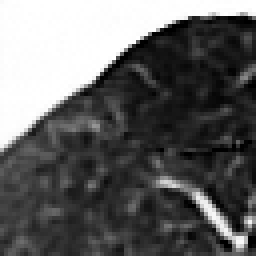
\includegraphics[width=18mm]{assets/healthy_patch.png}};
\node[caption, below=1.5mm of healthy] (healthyCap) {Healthy\\CT patch};

\node[imframe, right=9mm of healthy] (noise) {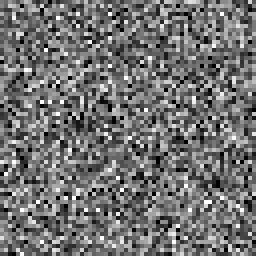
\includegraphics[width=18mm]{assets/noise_patch.png}};
\node[caption, below=1.5mm of noise] (noiseCap) {Noise};

\node[trainnet, right=9mm of noise] (rf) {3D Rectified\\Flow Network};
\node[block, right=8mm of rf] (loss) {Velocity\\Loss};

\node[imframe, right=8mm of loss] (priorImg) {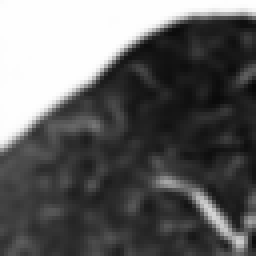
\includegraphics[width=18mm]{assets/learned_prior.png}};
\node[priorbox, below=1.5mm of priorImg] (prior) {Learned\\Healthy Prior};

\draw[arr] (healthy) -- (noise);
\draw[arr] (noise) -- (rf);
\draw[arr] (rf) -- (loss);
\draw[arr] (loss) -- (priorImg);
\draw[arr] (priorImg) -- (prior);

%%%%%%%%%%%%%%%%%%%%%%%%%%%%%%%%%%%%%%%%%%%%%%%%%%%%%%%%%%%%
%% Divider
%%%%%%%%%%%%%%%%%%%%%%%%%%%%%%%%%%%%%%%%%%%%%%%%%%%%%%%%%%%%
\draw[dashed, TrainBlue!35, thick] (-1.2, 2.55) -- (18.4, 2.55);

%%%%%%%%%%%%%%%%%%%%%%%%%%%%%%%%%%%%%%%%%%%%%%%%%%%%%%%%%%%%
%% INFERENCE
%%%%%%%%%%%%%%%%%%%%%%%%%%%%%%%%%%%%%%%%%%%%%%%%%%%%%%%%%%%%
\node[section, fill=InferTeal] (inferbanner) at (8.6, 2.15) {Inference (online)};

\node[imframe] (ct) at (0, 0.35) {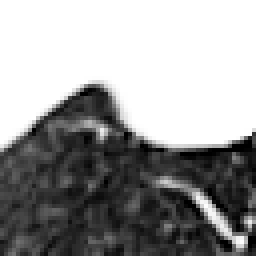
\includegraphics[width=17mm]{assets/test_ct.png}};
\node[caption, below=1.2mm of ct] {CT patch};

\node[imframe, right=6mm of ct] (box) {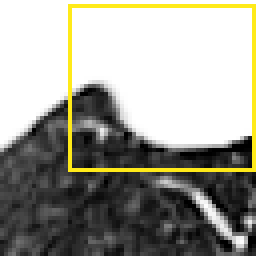
\includegraphics[width=17mm]{assets/box_prompt.png}};
\node[caption, below=1.2mm of box] {Box prompt};

\node[imframe, right=6mm of box] (hole) {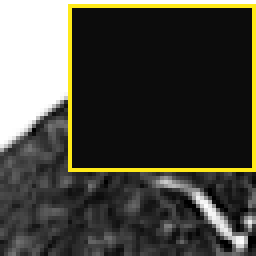
\includegraphics[width=17mm]{assets/initial_hole.png}};
\node[caption, below=1.2mm of hole] (holeCap) {Initial hole};

\node[network, right=7mm of hole] (inpaint) {Mask-guided\\Rectified Flow\\Inpainting};

\node[imframe, right=7mm of inpaint] (recon) {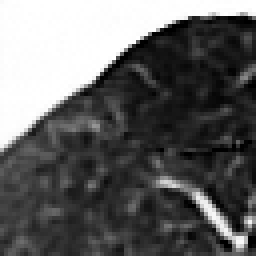
\includegraphics[width=17mm]{assets/healthy_reconstruction.png}};
\node[caption, below=1.2mm of recon] {Healthy recon.};

\node[imframe, right=6mm of recon] (resid) {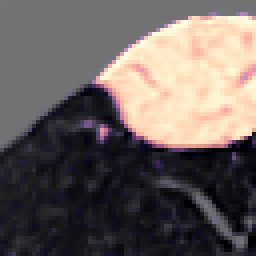
\includegraphics[width=17mm]{assets/residual.png}};
\node[caption, below=1.2mm of resid] {Residual\\$|x-\hat{x}|$};

\node[block, right=6mm of resid] (update) {Threshold\\+ refine};

\node[imframe, right=6mm of update] (seg) {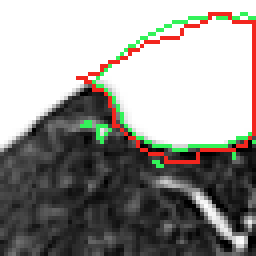
\includegraphics[width=17mm]{assets/final_seg.png}};
\node[outbox, below=1.2mm of seg] (segLab) {Final\\segmentation};

% main inference arrows (through image centers / blocks)
\draw[arr] (ct) -- (box);
\draw[arr] (box) -- (hole);
\draw[arr] (hole) -- (inpaint);
\draw[arr] (inpaint) -- (recon);
\draw[arr] (recon) -- (resid);
\draw[arr] (resid) -- (update);
\draw[arr] (update) -- (seg);
\draw[arr] (seg) -- (segLab);

%%%%%%%%%%%%%%%%%%%%%%%%%%%%%%%%%%%%%%%%%%%%%%%%%%%%%%%%%%%%
%% Prior → inpainting
%%%%%%%%%%%%%%%%%%%%%%%%%%%%%%%%%%%%%%%%%%%%%%%%%%%%%%%%%%%%
\draw[priorarr]
  (prior.south) to[out=-90, in=90]
  node[midway, right, font=\sffamily\scriptsize\itshape, text=TrainBlue] {use prior}
  (inpaint.north);

%%%%%%%%%%%%%%%%%%%%%%%%%%%%%%%%%%%%%%%%%%%%%%%%%%%%%%%%%%%%
%% Iterative refinement loop
%%%%%%%%%%%%%%%%%%%%%%%%%%%%%%%%%%%%%%%%%%%%%%%%%%%%%%%%%%%%
\draw[looparr]
  (update.south) to[out=-95, in=-85]
  node[midway, below, font=\sffamily\scriptsize\bfseries, text=LoopAmber]
    {Iterative refinement ($R$ rounds)}
  (hole.south);

%%%%%%%%%%%%%%%%%%%%%%%%%%%%%%%%%%%%%%%%%%%%%%%%%%%%%%%%%%%%
%% Zoom / mask refinement inset
%%%%%%%%%%%%%%%%%%%%%%%%%%%%%%%%%%%%%%%%%%%%%%%%%%%%%%%%%%%%
\begin{scope}[shift={(13.55,-3.85)}]
  \node[
    draw=Ink!45,
    rounded corners=3pt,
    fill=yellow!6,
    inner sep=5pt,
    align=center,
  ] (zoom) {
    \begin{tabular}{@{}c@{}}
      {\sffamily\bfseries\footnotesize Mask refinement}\\[1.5mm]
      {\sffamily\scriptsize Iteration 1}\\[0.8mm]
      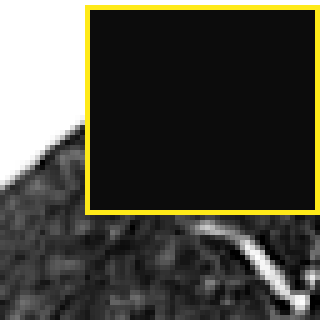
\includegraphics[width=28mm]{assets/iter1.png}\\[1.6mm]
      {\sffamily\scriptsize Residual}\\[0.8mm]
      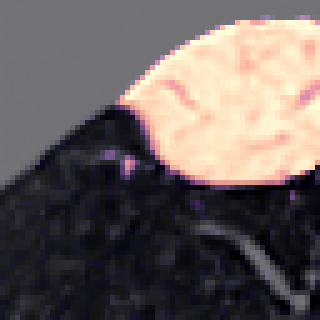
\includegraphics[width=28mm]{assets/residual1.png}\\[1.6mm]
      {\sffamily\scriptsize Iteration 2}\\[0.8mm]
      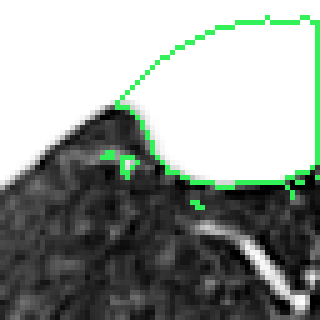
\includegraphics[width=28mm]{assets/iter2.png}\\[1.6mm]
      {\sffamily\scriptsize Final (red GT / lime pred)}\\[0.8mm]
      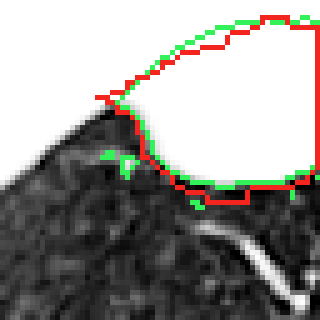
\includegraphics[width=28mm]{assets/final_zoom.png}
    \end{tabular}
  };
\end{scope}

% callout from update → zoom
\draw[arr, LoopAmber!80]
  (update.south east) to[out=-40, in=160]
  node[midway, above right, font=\sffamily\tiny, text=Muted] {detail}
  (zoom.north west);

%%%%%%%%%%%%%%%%%%%%%%%%%%%%%%%%%%%%%%%%%%%%%%%%%%%%%%%%%%%%
%% Footer
%%%%%%%%%%%%%%%%%%%%%%%%%%%%%%%%%%%%%%%%%%%%%%%%%%%%%%%%%%%%
\node[font=\sffamily\tiny, text=Muted, anchor=west]
  at (-1.1, -3.55)
  {Example LIDC patch \#1370 \;·\; red\,=\,GT, lime\,=\,prediction / residual foreground};

\end{tikzpicture}
\end{document}
